\documentclass{article}

\usepackage{tabularx}
\usepackage{booktabs}
\usepackage{array,multirow}
\usepackage{graphicx}
\title{Problem Statement and Goals\\\progname}

\author{\authname}

\date{}

%%% Comments

\usepackage{color}

\newif\ifcomments\commentstrue %displays comments
%\newif\ifcomments\commentsfalse %so that comments do not display

\ifcomments
\newcommand{\authornote}[3]{\textcolor{#1}{[#3 ---#2]}}
\newcommand{\todo}[1]{\textcolor{red}{[TODO: #1]}}
\else
\newcommand{\authornote}[3]{}
\newcommand{\todo}[1]{}
\fi

\newcommand{\wss}[1]{\authornote{blue}{SS}{#1}} 
\newcommand{\plt}[1]{\authornote{magenta}{TPLT}{#1}} %For explanation of the template
\newcommand{\an}[1]{\authornote{cyan}{Author}{#1}}

%%% Common Parts

\newcommand{\progname}{ProgName} % PUT YOUR PROGRAM NAME HERE
\newcommand{\authname}{Team \#, Team Name
\\ Student 1 name and macid
\\ Student 2 name and macid
\\ Student 3 name and macid
\\ Student 4 name and macid} % AUTHOR NAMES                  

\usepackage{hyperref}
    \hypersetup{colorlinks=true, linkcolor=blue, citecolor=blue, filecolor=blue,
                urlcolor=blue, unicode=false}
    \urlstyle{same}
                                


\begin{document}

\maketitle

\begin{table}[hp]
\caption{Revision History} \label{TblRevisionHistory}
\begin{tabularx}{\textwidth}{llX}
\toprule
\textbf{Date} & \textbf{Developer(s)} & \textbf{Change}\\
\midrule
Sept. 23, 2022 & Nicholas & Problem Statement\\\\
Sept. 25, 2022 & Longwei Ye & Problem Statement\\\\
Sept. 23, 2022 & Moksha Srinivasan & Goals, Stretch Goals\\
... & ... & ...\\
\bottomrule
\end{tabularx}
\end{table}
\newpage
\section{Problem Statement}



\subsection{Problem}
With the large usage of global positioning systems, software has been created to help researchers develop tools and methods based off peoples GPS data. 
One such software is the ArcPro toolbox that can match GPS traces to transportation networks. This software suffers from specific data requirements that limit usability, 
limited functionality and is not able to handle the use of larger GPS data sets. In order to overcome these weaknesses the ArcPro toolbox must be re-engineered with a focuses 
on transferability, modularity, and scalability as well as being open source without using any proprietary software. 

\subsection{Inputs and Outputs}
\begin{table}[h]
    \centering
    \begin{tabular}{|p{6cm}|p{6cm}|}
    \hline
    Input & Output  \\
    \hline
    \multirow{2}{5cm}{A dataset of latitude and longitude positions and times based on persons typical route during the day} & Identify sections of each travelers day based on the location they are in for some period of time.  \\\cline{2-2} 
    & Identify the travelers method of transportation they are using during each episode (See Definitions)  \\\cline{2-2} 
    & Estimate the possible route a traveler will take\\\cline{2-2} 
    \hline
    \end{tabular}
\end{table}

\subsection{Stakeholders}
Potential stakeholders in this project include any researchers and/or companies who are interested in matching GPS data to transportation networks in the context of travel episodes and route estimations analysis. 

\subsection{Environment}
yoGERT is an open-source toolbox that is able to run on personal laptops and desktops that uses Linux, Windows, and MacOS operating system 
with Python pre-installed.

\newpage
\section{Goals}
\begin{table}[h!]
    \centering
        \begin{tabular}{|p{6cm}|p{6cm}|}
    		\hline
    		\textbf{Goal} & \textbf{Importance} \\
    		\hline
    		The toolbox will be completely open-source without reliance on the proprietary ArcGIS or subsidiary software. & An open-source toolbox will allow a greater audience to process and use the abundance of GPS data that is collected every day. Additionally, it avoids dependency on expensive licensing required for proprietary ArcGIS Pro software. \\
    		\hline
    		The toolbox will quickly normalize and process common GPS file formats (GPRMC, GPGGA, GPGLL...) into compatible data types. & Similar to its predecessor, this toolbox aims to be highly flexible, allowing for a variety of input formats. Many existing tools are not input agnostic and as such cannot process a variety of data.  \\
    		\hline
    		The toolbox supports fast and accurate route choice model estimations. & Route choice model estimations are models of possible routes a traveler may take based on their intermediary GPS information. These models can be used for a variety of applications. Examples include; forecasting traveler behaviour and predicting future traffic conditions on transportation networks. \\
    		\hline
    		The toolbox will be able to extract travel episodes, identify stops, intermediary trip information, potential activity locations (PALs), and assign trip purposes to episodes. & Many existing tools are able to extract travel episodes and assign trip purposes. By extending the functionality to include stop identification, PALs, and parse intermediary trip information, the toolbox provides much requested functionality for researchers. \\
    		\hline
    		The toolbox will be able to process 47.3 million points of GPS data within at most 6000 seconds. & Similar to its predecessor, this toolbox aims to be highly scalable, with the ability to process large amounts of data in a short amount of time. This makes it more viable to use GPS data for applications that require regular processing of data.\\
    		\hline
    	\end{tabular}
		
\end{table}


\section{Stretch Goals}

\begin{tabular}{|p{6cm}|p{6cm}|}
    		\hline
    		\textbf{Goal} & \textbf{Importance} \\
    		\hline
    		The toolbox will contain functionality to teach students about data processing methods, and develop intuition for how episodes are categorized. & This will allow the toolbox to be both a data processor as well as a learning tool for those who are new to GPS data analysis.  \\
    		\hline
    		The toolbox will provide an interactive GUI with map overlays for episodes and corresponding information. & The toolbox will not only provide graphs based on inputs and desired outputs, but users will also be able to understand how the density of data points change for different episodes.  \\
    		\hline
\end{tabular}
\section{Definitions}
%[1] 
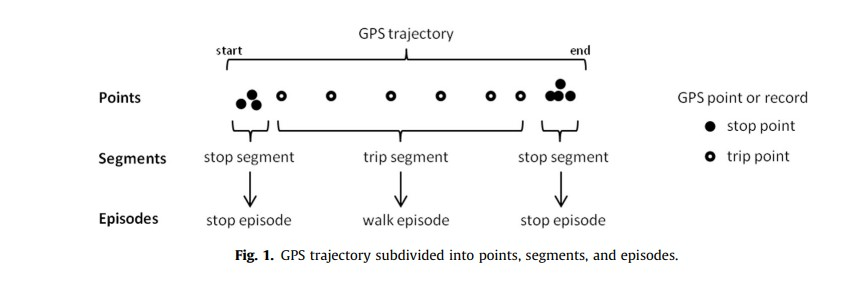
\includegraphics[scale=0.6]{REV0/ProblemStatementAndGoals/gert.jpg}
\subsection{Episodes}
In the context of activity analysis, a person’s 24-h (daily) activities can be subdivided into episodes, which are differentiated
based on location (inside a building or travel mode); hence an
activity episode can be a stationary episode (stop episode) or a travel episode (e.g., car episode). [1]

\section{Bibliography}
\begin{itemize}
    \item $[1]$ R. Dalumpines and D. M. Scott, “GIS-based episode Reconstruction Toolkit (Gert): A transferable, modular, and scalable framework for automated extraction of activity episodes from GPS Data,” Travel Behaviour and Society, vol. 11, pp. 121–130, 2018. 
\end{itemize}
 
\end{document}
